\documentclass[aspectratio=169,11pt]{beamer}
\usetheme{metropolis}
\usepackage{tikz}
\usetikzlibrary{arrows.meta,positioning,calc}
\usepackage{booktabs}
\usepackage{array}
\usepackage{xcolor}
\usepackage{amsmath}
\usepackage{hyperref}

% === Color palette ===
\definecolor{report}{HTML}{3498DB}
\definecolor{state}{HTML}{9B59B6}
\definecolor{bias}{HTML}{E67E22}
\definecolor{neutral}{HTML}{95A5A6}
\definecolor{pass}{HTML}{27AE60}
\definecolor{fail}{HTML}{E74C3C}
\tikzset{
  box/.style={draw=#1,thick,rounded corners,fill=#1!10,minimum width=3.2cm,minimum height=0.9cm,font=\small,align=center},
  boxL/.style={draw=#1,thick,rounded corners,fill=#1!10,minimum width=5.2cm,minimum height=1.2cm,font=\small,align=center},
  boxS/.style={draw=#1,thick,rounded corners,fill=#1!10,minimum width=2.8cm,minimum height=0.9cm,font=\footnotesize,align=center},
  cell/.style={draw=#1,thick,rounded corners,fill=#1!10,minimum width=3.6cm,minimum height=1.1cm,font=\small,align=center},
}
\hypersetup{colorlinks=true,linkcolor=.,urlcolor=report}

% Title page: metropolis sizes its minipage to \paperheight, which overflows the frame.
\makeatletter
\setbeamertemplate{title page}{
  \begin{minipage}[b][\dimexpr\paperheight-16pt\relax]{\textwidth}
    \vfill%
    \usebeamertemplate*{title}
    \usebeamertemplate*{subtitle}
    \usebeamertemplate*{title separator}
    \usebeamertemplate*{author}
    \vfill
    \vspace*{1mm}
  \end{minipage}
}
\makeatother

\newcommand{\FL}{\href{https://www.frontiersin.org/articles/10.3389/fnhum.2014.00443/pdf}{Fleming \& Lau 2014}}
\newcolumntype{L}[1]{>{\raggedright\arraybackslash}p{#1}}
\newcommand{\site}{https://measuring-introspection.github.io/measuring-introspection}

\title{Signal Detection and Metacognition}
\subtitle{Sensitivity, bias and confidence, applied to LLM introspection}
\author{Measuring AI Introspection}
\date{}
\institute{}

\newcommand{\partslide}[2]{%
\begin{frame}[plain,label=#1]
\vfill
\begin{center}
  \setlength{\fboxrule}{2.5pt}%
  \fcolorbox{black}{white}{\parbox{0.65\textwidth}{\centering\vspace{0.8em}
    {\Large\bfseries #2}
  \vspace{0.8em}}}
\end{center}
\vfill
\end{frame}}

\begin{document}

\maketitle

%% --- Overview ---
\begin{frame}{Overview}\footnotesize
\begin{columns}[T]
\begin{column}{0.48\textwidth}
\hyperlink{part1}{\textbf{Part 1: Sensitivity and saying yes}}\\[0.15em]
{\scriptsize%
\quad\hyperlink{running}{1.~The running example}\\%
\quad\hyperlink{fourout}{2.~Four outcomes}\\%
\quad\hyperlink{curves}{3.~Two bell curves and a line}\\%
\quad\hyperlink{samehit}{4.~Same hit rate, different observers}\\%
\quad\hyperlink{formulas}{5.~Sensitivity and criterion as numbers}%
}\vspace{0.15em}

\hyperlink{part2}{\textbf{Part 2: Confidence about one's own answers}}\\[0.15em]
{\scriptsize%
\quad\hyperlink{types}{6.~Type-1 and type-2 tasks}\\%
\quad\hyperlink{table2}{7.~The confidence-accuracy table}\\%
\quad\hyperlink{three}{8.~Sensitivity, bias and efficiency}\\%
\quad\hyperlink{fail}{9.~Correlations and type-2 $d'$}\\%
\quad\hyperlink{auroc}{10.~AUROC2}\\%
\quad\hyperlink{metad}{11.~Meta-$d'$ and the M-ratio}%
}
\end{column}
\begin{column}{0.48\textwidth}
\hyperlink{part3}{\textbf{Part 3: Probabilities and awareness}}\\[0.15em]
{\scriptsize%
\quad\hyperlink{brier}{12.~The Brier decomposition}\\%
\quad\hyperlink{calsenses}{13.~Three senses of calibration}\\%
\quad\hyperlink{michel}{14.~Michel's four conditions}%
}\vspace{0.15em}

\hyperlink{part4}{\textbf{Part 4: Language models}}\\[0.15em]
{\scriptsize%
\quad\hyperlink{injection}{15.~Concept injection as a type-1 task}\\%
\quad\hyperlink{hahami}{16.~Injection moves the criterion}\\%
\quad\hyperlink{logit}{17.~A logit as a decision variable}\\%
\quad\hyperlink{conftasks}{18.~Confidence papers as type-2 tasks}\\%
\quad\hyperlink{probe}{19.~A probe as the ideal observer}%
}\vspace{0.15em}

\hyperlink{part5}{\textbf{Part 5: Limits}}\\[0.15em]
{\scriptsize%
\quad\hyperlink{limits}{20.~Where the analogy stops}\\%
\quad\hyperlink{summary}{21.~Summary}\\%
\quad\hyperlink{reading}{22.~Reading}%
}
\end{column}
\end{columns}
\end{frame}

%% ============================================================
\partslide{part1}{Part 1\\[0.5em]{\large\mdseries Sensitivity and saying yes}}
%% ============================================================

\begin{frame}[label=running]{The running example}
\href{\site/papers/lindsey-2025/}{Lindsey (2025)} runs a \emph{concept injection} experiment:

\vspace{0.3em}
\begin{enumerate}\setlength\itemsep{3pt}
  \item {\small Take the model's internal activation pattern for a word, such as \emph{bread}.}
  \item {\small Add it to the model's activations on some trials, and leave the activations alone on others.}
  \item {\small Ask: \emph{Do you detect an injected thought?}}
\end{enumerate}

\vspace{0.3em}
\begin{center}
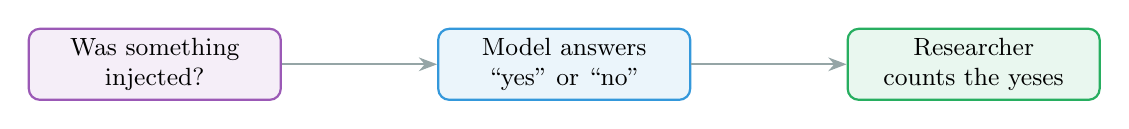
\begin{tikzpicture}
  \node[box=state] (inj) at (0,0) {Was something\\injected?};
  \node[box=report] (ans) at (5.2,0) {Model answers\\``yes'' or ``no''};
  \node[box=pass] (score) at (10.4,0) {Researcher\\counts the yeses};
  \draw[-{Stealth},thick,neutral] (inj) -- (ans);
  \draw[-{Stealth},thick,neutral] (ans) -- (score);
\end{tikzpicture}
\end{center}

\vspace{0.3em}
{\small Signal detection theory is the standard way to read a pile of yes/no answers. It splits a rate of ``yes'' into two things: how well the model tells injection from no injection, and how willing it is to say yes.}
\end{frame}

\begin{frame}[label=fourout]{Four outcomes}
Every trial lands in one of four cells:

\vspace{0.2em}
\begin{center}
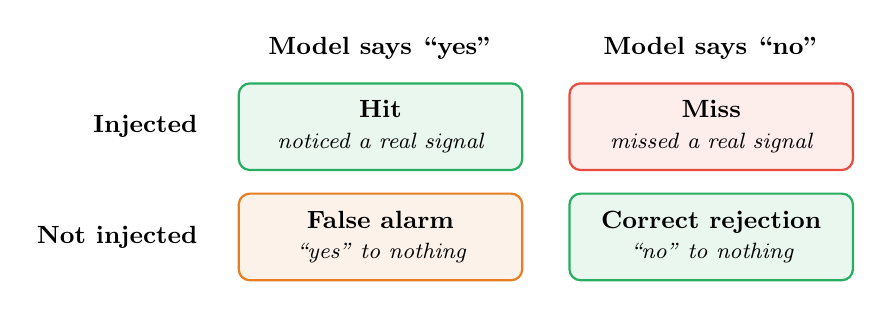
\begin{tikzpicture}
  \node[font=\small\bfseries] at (3,1.0) {Model says ``yes''};
  \node[font=\small\bfseries] at (7.2,1.0) {Model says ``no''};
  \node[font=\small\bfseries,anchor=east] at (0.8,0) {Injected};
  \node[font=\small\bfseries,anchor=east] at (0.8,-1.4) {Not injected};
  \node[cell=pass] at (3,0) {\textbf{Hit}\\{\footnotesize\itshape noticed a real signal}};
  \node[cell=fail] at (7.2,0) {\textbf{Miss}\\{\footnotesize\itshape missed a real signal}};
  \node[cell=bias] at (3,-1.4) {\textbf{False alarm}\\{\footnotesize\itshape ``yes'' to nothing}};
  \node[cell=pass] at (7.2,-1.4) {\textbf{Correct rejection}\\{\footnotesize\itshape ``no'' to nothing}};
\end{tikzpicture}
\end{center}

\vspace{0.3em}
The \textbf{hit rate} $H$ is the share of ``yes'' on injected trials. The \textbf{false-alarm rate} $F$ is the share of ``yes'' on trials with nothing injected.

\vspace{0.2em}
{\small Each row needs its own trials, and both rows are needed.}
\end{frame}

\begin{frame}[label=curves]{Two bell curves and a line}
\begin{columns}[T]
\begin{column}{0.55\textwidth}
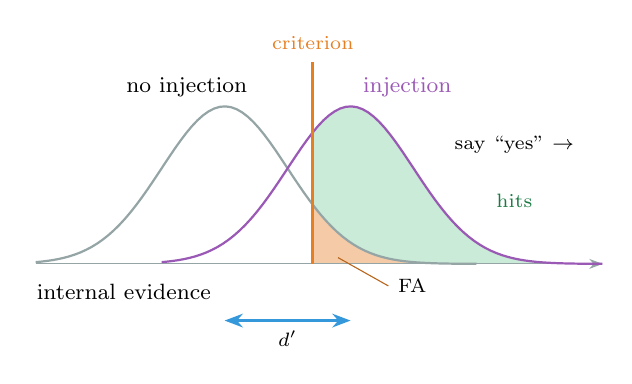
\begin{tikzpicture}[scale=0.8]
  \fill[bias!25,domain=1.4:4,samples=40] (1.4,0) -- plot (\x,{2.5*exp(-(\x)^2/2)}) -- (4,0) -- cycle;
  \fill[pass!25,domain=1.4:6,samples=60] (1.4,0) -- plot (\x,{2.5*exp(-(\x-2)^2/2)}) -- (6,0) -- cycle;
  \fill[bias!40,domain=1.4:4,samples=40] (1.4,0) -- plot (\x,{2.5*exp(-(\x)^2/2)}) -- (4,0) -- cycle;
  \draw[-{Stealth},neutral] (-3,0) -- (6,0);
  \node[font=\footnotesize,text=black] at (-1.6,-0.45) {internal evidence};
  \draw[thick,neutral,domain=-3:4,samples=80] plot (\x,{2.5*exp(-(\x)^2/2)});
  \draw[thick,state,domain=-1:6,samples=80] plot (\x,{2.5*exp(-(\x-2)^2/2)});
  \node[font=\footnotesize,text=black] at (-0.6,2.8) {no injection};
  \node[font=\footnotesize,state] at (2.9,2.8) {injection};
  \draw[bias,very thick] (1.4,0) -- (1.4,3.2);
  \node[font=\scriptsize,bias,align=center] at (1.4,3.5) {criterion};
  \node[font=\scriptsize] at (4.6,1.9) {say ``yes'' $\rightarrow$};
  \node[font=\scriptsize] at (4.6,1.0) {\textcolor{pass!70!black}{hits}};
  \draw[bias!80!black] (1.8,0.1) -- (2.6,-0.35) node[right,font=\scriptsize,text=black]{FA};
  \draw[{Stealth}-{Stealth},report,thick] (0,-0.9) -- node[below,font=\scriptsize,text=black]{$d'$} (2,-0.9);
\end{tikzpicture}
\end{column}
\begin{column}{0.43\textwidth}
{\small
On each trial the model has some amount of internal evidence. It varies from trial to trial, so each condition gives a bell curve.

\vspace{0.4em}
\textbf{\textcolor{report}{Sensitivity}} ($d'$): how far apart the two curves are.

\vspace{0.4em}
\textbf{\textcolor{bias}{Criterion}}: the line. Evidence to the right of it gets a ``yes''.

\vspace{0.4em}
Green area: hits. Orange area: false alarms (FA).
}
\end{column}
\end{columns}
\end{frame}

\begin{frame}[label=samehit]{Same hit rate, different observers}
\begin{columns}[T]
\begin{column}{0.48\textwidth}
\begin{center}
{\small\textbf{High sensitivity, strict criterion}}\\[0.3em]
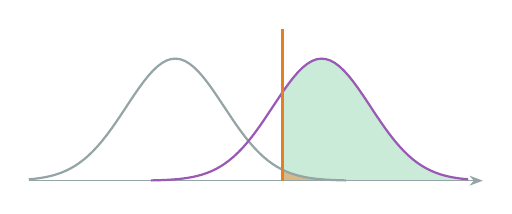
\begin{tikzpicture}[scale=0.62]
  \fill[pass!25,domain=2.2:6,samples=50] (2.2,0) -- plot (\x,{2.5*exp(-(\x-3)^2/2)}) -- (6,0) -- cycle;
  \fill[bias,fill opacity=0.45,domain=2.2:3.5,samples=30] (2.2,0) -- plot (\x,{2.5*exp(-(\x)^2/2)}) -- (3.5,0) -- cycle;
  \draw[-{Stealth},neutral] (-3,0) -- (6.3,0);
  \draw[thick,neutral,domain=-3:3.5,samples=70] plot (\x,{2.5*exp(-(\x)^2/2)});
  \draw[thick,state,domain=-0.5:6,samples=70] plot (\x,{2.5*exp(-(\x-3)^2/2)});
  \draw[bias,very thick] (2.2,0) -- (2.2,3.1);
\end{tikzpicture}\\[0.2em]
{\footnotesize Curves far apart; line far right.\\Almost no false alarms.}
\end{center}
\end{column}
\begin{column}{0.48\textwidth}
\begin{center}
{\small\textbf{Low sensitivity, lax criterion}}\\[0.3em]
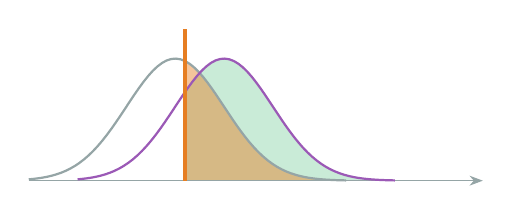
\begin{tikzpicture}[scale=0.62]
  \fill[pass!25,domain=0.2:4.5,samples=50] (0.2,0) -- plot (\x,{2.5*exp(-(\x-1)^2/2)}) -- (4.5,0) -- cycle;
  \fill[bias,fill opacity=0.45,domain=0.2:3.5,samples=40] (0.2,0) -- plot (\x,{2.5*exp(-(\x)^2/2)}) -- (3.5,0) -- cycle;
  \draw[-{Stealth},neutral] (-3,0) -- (6.3,0);
  \draw[thick,neutral,domain=-3:3.5,samples=70] plot (\x,{2.5*exp(-(\x)^2/2)});
  \draw[thick,state,domain=-2:4.5,samples=70] plot (\x,{2.5*exp(-(\x-1)^2/2)});
  \draw[bias,very thick] (0.2,0) -- (0.2,3.1);
\end{tikzpicture}\\[0.2em]
{\footnotesize Curves overlap; line far left.\\Many false alarms (orange).}
\end{center}
\end{column}
\end{columns}

\vspace{0.5em}
Both observers say ``yes'' on the same share of injected trials. One is sharp and cautious; the other barely tells the conditions apart and says yes readily.

\vspace{0.3em}
{\small A hit rate alone cannot tell them apart. Only the false-alarm rate can.}
\end{frame}

\begin{frame}[label=formulas]{Sensitivity and criterion as numbers}
Under the equal-variance Gaussian model:
\[
d' = z(H) - z(F) \qquad\qquad c = -\tfrac{1}{2}\,\bigl[z(H) + z(F)\bigr]
\]

{\small $z$ turns a rate into a position on the bell curve, measured in standard deviations (the inverse of the standard normal cumulative distribution function).}

\vspace{0.5em}
\begin{center}
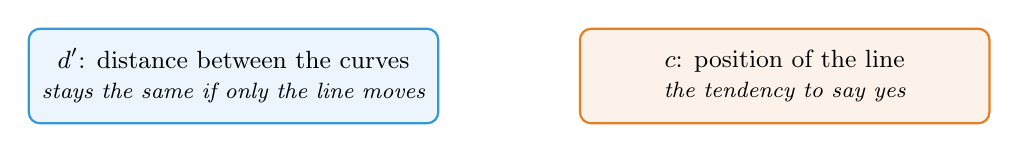
\begin{tikzpicture}
  \node[boxL=report] (d) at (0,0) {$d'$: distance between the curves\\{\footnotesize\itshape stays the same if only the line moves}};
  \node[boxL=bias] (c) at (7,0) {$c$: position of the line\\{\footnotesize\itshape the tendency to say yes}};
\end{tikzpicture}
\end{center}

\vspace{0.5em}
{\small Percentage correct mixes the two. $d'$ stays constant when only the criterion changes (\FL).}
\end{frame}

%% ============================================================
\partslide{part2}{Part 2\\[0.5em]{\large\mdseries Confidence about one's own answers}}
%% ============================================================

\begin{frame}[label=types]{Type-1 and type-2 tasks}
Metacognition research applies the same split one level up, to confidence.

\vspace{0.6em}
\begin{center}
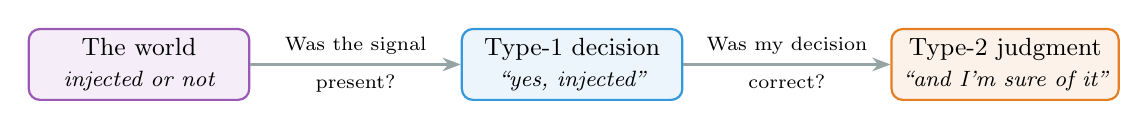
\begin{tikzpicture}
  \node[box=state,minimum width=2.8cm] (w) at (0,0) {The world\\{\footnotesize\itshape injected or not}};
  \node[box=report,minimum width=2.8cm] (d) at (5.5,0) {Type-1 decision\\{\footnotesize\itshape ``yes, injected''}};
  \node[box=bias,minimum width=2.8cm] (c) at (11.0,0) {Type-2 judgment\\{\footnotesize\itshape ``and I'm sure of it''}};
  \draw[-{Stealth},thick,neutral] (w) -- node[above,font=\scriptsize,text=black]{Was the signal} node[below,font=\scriptsize,text=black]{present?} (d);
  \draw[-{Stealth},thick,neutral] (d) -- node[above,font=\scriptsize,text=black]{Was my decision} node[below,font=\scriptsize,text=black]{correct?} (c);
\end{tikzpicture}
\end{center}

\vspace{0.6em}
A \textbf{type-1} task asks about the world. A \textbf{type-2} task asks about the observer's own type-1 decision.

\vspace{0.3em}
{\small The type-2 score is checked against whether the observer was right, not against the state of the world (\FL).}
\end{frame}

\begin{frame}[label=table2]{The confidence-accuracy table}
Same four cells as before, one level up. Rows are now \emph{was I right}, columns are \emph{how sure was I}:

\vspace{0.5em}
\begin{center}
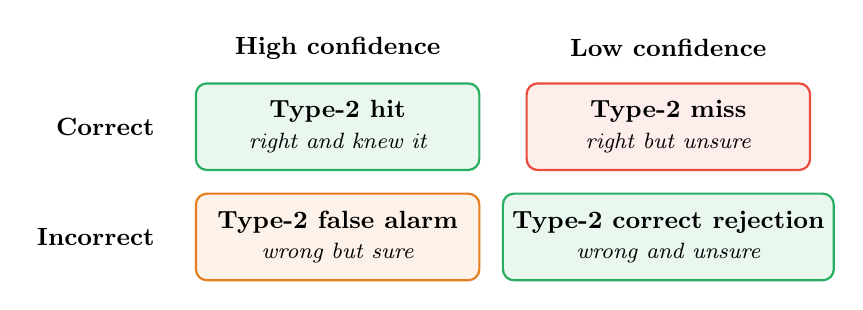
\begin{tikzpicture}
  \node[font=\small\bfseries] at (3,1.0) {High confidence};
  \node[font=\small\bfseries] at (7.2,1.0) {Low confidence};
  \node[font=\small\bfseries,anchor=east] at (0.8,0) {Correct};
  \node[font=\small\bfseries,anchor=east] at (0.8,-1.4) {Incorrect};
  \node[cell=pass] at (3,0) {\textbf{Type-2 hit}\\{\footnotesize\itshape right and knew it}};
  \node[cell=fail] at (7.2,0) {\textbf{Type-2 miss}\\{\footnotesize\itshape right but unsure}};
  \node[cell=bias] at (3,-1.4) {\textbf{Type-2 false alarm}\\{\footnotesize\itshape wrong but sure}};
  \node[cell=pass] at (7.2,-1.4) {\textbf{Type-2 correct rejection}\\{\footnotesize\itshape wrong and unsure}};
\end{tikzpicture}
\end{center}

\vspace{0.5em}
{\small Good metacognition fills the green cells: confidence is high when the decision was right and low when it was wrong.}
\end{frame}

\begin{frame}[label=three]{Sensitivity, bias and efficiency}
Three quantities are defined on this table (\FL):

\vspace{0.5em}
\begin{center}
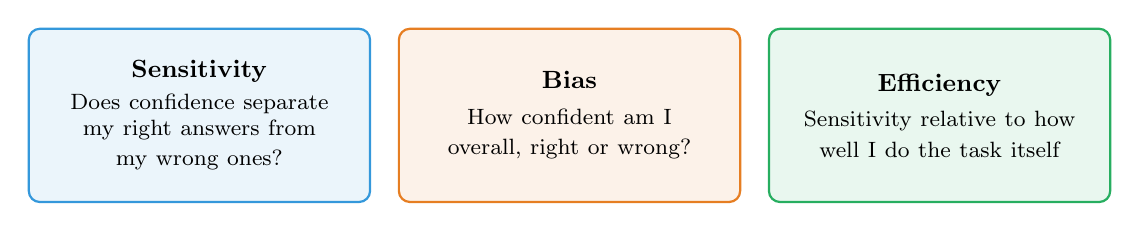
\begin{tikzpicture}
  \node[box=report,minimum width=4.3cm,minimum height=2.2cm,text width=4.1cm] at (0,0) {\textbf{Sensitivity}\\[0.2em]{\footnotesize Does confidence separate\\my right answers from\\my wrong ones?}};
  \node[box=bias,minimum width=4.3cm,minimum height=2.2cm,text width=4.1cm] at (4.7,0) {\textbf{Bias}\\[0.2em]{\footnotesize How confident am I overall, right or wrong?}};
  \node[box=pass,minimum width=4.3cm,minimum height=2.2cm,text width=4.1cm] at (9.4,0) {\textbf{Efficiency}\\[0.2em]{\footnotesize Sensitivity relative to how well I do the task itself}};
\end{tikzpicture}
\end{center}

\vspace{0.5em}
{\small Bias is also called over- or underconfidence, or calibration. Sensitivity is also called metacognitive accuracy or discrimination.}

\vspace{0.3em}
{\small A subject can be confident overall and still have poor sensitivity, if confidence is equally high on correct and incorrect trials.}
\end{frame}

\begin{frame}[label=fail]{Correlations and type-2 $d'$}
\FL\ review the obvious measures of metacognitive sensitivity. Two families fail:

\vspace{0.4em}
\begin{center}
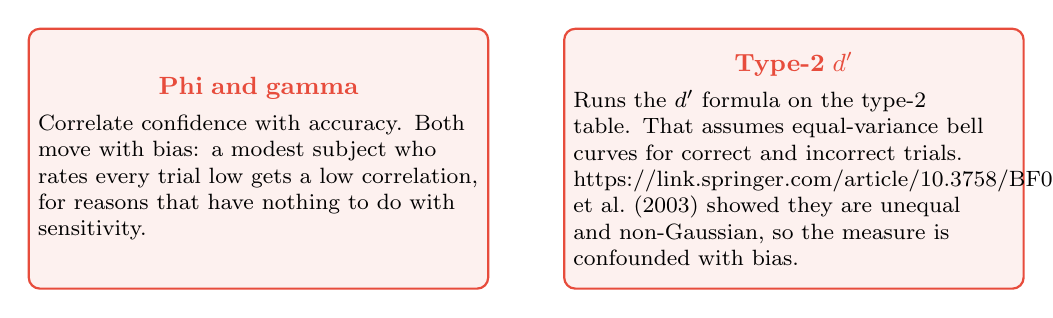
\begin{tikzpicture}
  \node[draw=fail,thick,rounded corners,fill=fail!8,text width=5.6cm,minimum height=3.3cm,align=left,anchor=north,font=\footnotesize] at (0,0) {{\centering\small\bfseries\textcolor{fail}{Phi and gamma}\par}\vspace{0.4em}Correlate confidence with accuracy. Both move with bias: a modest subject who rates every trial low gets a low correlation, for reasons that have nothing to do with sensitivity.};
  \node[draw=fail,thick,rounded corners,fill=fail!8,text width=5.6cm,minimum height=3.3cm,align=left,anchor=north,font=\footnotesize] at (6.8,0) {{\centering\small\bfseries\textcolor{fail}{Type-2 $d'$}\par}\vspace{0.4em}Runs the $d'$ formula on the type-2 table. That assumes equal-variance bell curves for correct and incorrect trials. \href{https://link.springer.com/article/10.3758/BF03196546}{Galvin et al.\ (2003)} showed they are unequal and non-Gaussian, so the measure is confounded with bias.};
\end{tikzpicture}
\end{center}

\vspace{0.4em}
{\small Both fail the same way: a change in how confident the subject is overall shows up as a change in sensitivity.}
\end{frame}

\begin{frame}[label=auroc]{AUROC2}
\begin{columns}[T]
\begin{column}{0.46\textwidth}
\begin{center}
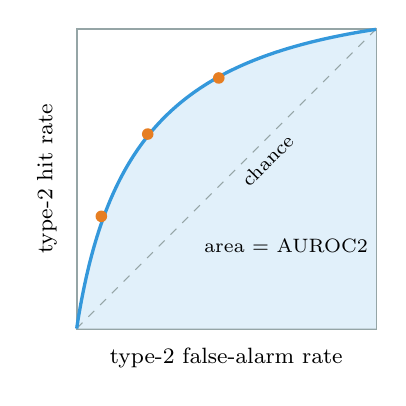
\begin{tikzpicture}[scale=0.95]
  \draw[neutral,thick] (0,0) rectangle (4,4);
  \fill[report!15] (0,0) .. controls (0.4,2.6) and (1.4,3.6) .. (4,4) -- (4,0) -- cycle;
  \draw[neutral,dashed] (0,0) -- (4,4);
  \draw[report,very thick] (0,0) .. controls (0.4,2.6) and (1.4,3.6) .. (4,4);
  \foreach \p in {(0.33,1.5),(0.95,2.6),(1.9,3.35)} \fill[bias] \p circle (2.2pt);
  \node[font=\footnotesize,text=black] at (2,-0.4) {type-2 false-alarm rate};
  \node[font=\footnotesize,text=black,rotate=90] at (-0.4,2) {type-2 hit rate};
  \node[font=\scriptsize,text=black] at (2.8,1.1) {area = AUROC2};
  \node[font=\scriptsize,text=black,rotate=45] at (2.55,2.25) {chance};
\end{tikzpicture}
\end{center}
\end{column}
\begin{column}{0.5\textwidth}
{\small
Treat each confidence level as a criterion. Each one gives a point: a type-2 hit rate and a type-2 false-alarm rate (\textcolor{bias}{orange dots}).

\vspace{0.4em}
Join the points into a curve. The area under it is \textbf{AUROC2}. The diagonal is confidence that says nothing about correctness.

\vspace{0.4em}
\textcolor{pass}{\textbf{Good:}} free of bias.

\vspace{0.2em}
\textcolor{fail}{\textbf{Problem:}} it rises with task performance. The same subject scores higher on an easy task than on a hard one.
}
\end{column}
\end{columns}
\end{frame}

\begin{frame}[label=metad]{Meta-$d'$ and the M-ratio}
\relax{\small \textbf{Meta-$d'$} (\href{https://www.sciencedirect.com/science/article/abs/pii/S1053810011002303}{Maniscalco \& Lau 2012}): the $d'$ that an ideal observer, one who uses all the evidence, would need to produce the confidence performance actually seen. Same units as $d'$, so the two compare directly.}

\vspace{-0.1em}
\begin{center}
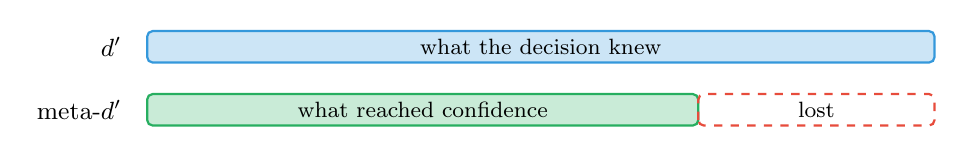
\begin{tikzpicture}
  \node[font=\small,anchor=east] at (-0.2,0.35) {$d'$};
  \node[font=\small,anchor=east] at (-0.2,-0.45) {meta-$d'$};
  \fill[report!25,draw=report,thick,rounded corners=2pt] (0,0.15) rectangle (10,0.55);
  \node[font=\footnotesize] at (5,0.35) {what the decision knew};
  \fill[pass!25,draw=pass,thick,rounded corners=2pt] (0,-0.65) rectangle (7,-0.25);
  \node[font=\footnotesize] at (3.5,-0.45) {what reached confidence};
  \draw[fail,thick,dashed,rounded corners=2pt] (7,-0.65) rectangle (10,-0.25);
  \node[font=\footnotesize,text=black] at (8.5,-0.45) {lost};
\end{tikzpicture}
\end{center}

\vspace{0.1em}
{\small \textbf{M-ratio} $=$ meta-$d'/d'$: how much of what you know reaches your confidence.\\[0.2em]
\textcolor{pass}{\textbf{M-ratio $=1$}}: a metacognitively ideal observer; all the evidence reached confidence.\\[0.1em]
\textcolor{fail}{\textbf{M-ratio $=0.7$}}: 30\% of the evidence was lost on the way to confidence (\FL).}

\vspace{0.2em}
{\footnotesize \href{https://philarchive.org/archive/MICCIC-3}{Michel (2023)} calls the M-ratio the gold standard for metacognitive efficiency. When $d'$ is small the ratio is unstable, and meta-$d'-d'$ or the log ratio is used instead.}
\end{frame}

%% ============================================================
\partslide{part3}{Part 3\\[0.5em]{\large\mdseries Probabilities and awareness}}
%% ============================================================

\begin{frame}[label=brier]{The Brier decomposition}
A stated probability gives bias an absolute scale: a stated 70\% can be checked against the proportion correct. The Brier score, the mean squared gap between stated probability and outcome, splits as
\vspace{-0.3em}
\[
PS = \underbrace{O}_{\text{outcome variance}} + \underbrace{C}_{\text{calibration}} - \underbrace{R}_{\text{resolution}}
\]

\vspace{-0.3em}
\begin{center}
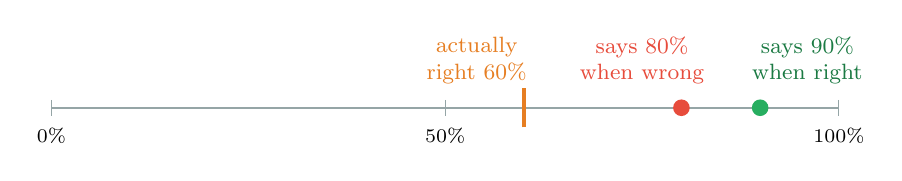
\begin{tikzpicture}
  \draw[neutral,thick] (0,0) -- (10,0);
  \foreach \x/\l in {0/0\%,5/50\%,10/100\%} {\draw[neutral] (\x,0.1) -- (\x,-0.1); \node[font=\scriptsize,text=black] at (\x,-0.35) {\l};}
  \fill[pass] (9,0) circle (3pt); \node[font=\footnotesize,pass!70!black,align=center] at (9.6,0.6) {says 90\%\\when right};
  \fill[fail] (8,0) circle (3pt); \node[font=\footnotesize,fail,align=center] at (7.5,0.6) {says 80\%\\when wrong};
  \draw[bias,very thick] (6,-0.25) -- (6,0.25); \node[font=\footnotesize,bias,align=center] at (5.4,0.6) {actually\\right 60\%};
\end{tikzpicture}
\end{center}

\vspace{-0.8em}
{\small
\textbf{Calibration} (bias): poor; both confidence levels sit far above 60\%.
\textbf{Resolution} (sensitivity): good. Right answers always get more confidence than wrong ones (\FL).}

{\footnotesize Because $O$ depends on accuracy, the Brier score moves with task performance.}
\end{frame}

\begin{frame}[label=calsenses]{Three senses of calibration}
Papers on LLM introspection use ``calibration'' in more than one sense:

\vspace{0.2em}
\begin{center}
{\footnotesize\renewcommand{\arraystretch}{1.15}
\begin{tabular}{L{2.8cm}L{6.2cm}L{3.6cm}}
\toprule
\textbf{Sense} & \textbf{Meaning} & \textbf{Where it appears} \\
\midrule
\textcolor{state}{\textbf{Metrological}} & Relating an instrument's indications to values of the measurand, against a standard & \href{\site/foundations/metrology/}{Metrology} \\
\textcolor{bias}{\textbf{Probability}} & Stated confidence agrees with proportion correct; the $C$ term of the Brier score & Kadavath et al.'s expected calibration error; Ferrara's Brier score \\
\textcolor{report}{\textbf{Discriminatory}} & Confidence rank-orders outcomes; metacognitive sensitivity under another name & Moran and Whiting, Def.~3.1 \\
\bottomrule
\end{tabular}
}
\end{center}

\vspace{0.2em}
{\small \href{\site/papers/kadavath-2022/}{Kadavath et al.\ (2022)} state the difference between the second and third: the area under the curve measures discrimination and ignores calibration.}
\end{frame}

\begin{frame}[label=michel]{Michel's four conditions}
\relax{\small \href{https://philarchive.org/archive/MICCIC-3}{Michel (2023)} separates \textbf{validity} (does the procedure measure the intended attribute?) from \textbf{accuracy} (how well?), and states four conditions:}

\begin{center}
{\footnotesize\renewcommand{\arraystretch}{1.0}
\begin{tabular}{L{3.4cm}L{7.2cm}L{1.8cm}}
\toprule
\textbf{Condition} & \textbf{Content} & \textbf{Guarantees} \\
\midrule
Consciousness-selectivity & Unconscious sensory activity is a source of metacognitive inefficiency & \textcolor{pass}{\textbf{Validity}} \\
Optimal metacognition & Metacognition is optimal for decisions based on conscious activity & \textcolor{report}{\textbf{Accuracy}} \\
No overflow & All conscious activity is available for metacognitive decisions & \textcolor{report}{\textbf{Accuracy}} \\
No hallucination & Activity driving false alarms is not conscious & \textcolor{report}{\textbf{Accuracy}} \\
\bottomrule
\end{tabular}
}
\end{center}

\vspace{0.1em}
{\small Other sources of inefficiency are confounds. Controls: remove them (\emph{ceteris absentibus}), equate them across conditions (\emph{ceteris paribus}), or make them negligible (\emph{ceteris neglectis}).}
\end{frame}

%% ============================================================
\partslide{part4}{Part 4\\[0.5em]{\large\mdseries Language models}}
%% ============================================================

\begin{frame}[label=injection]{Concept injection as a type-1 task}
\relax{\small The stimulus is internal, but the question is type-1: was a signal present?}

\vspace{0.1em}
\begin{center}

\begin{tikzpicture}
  \node[box=pass,minimum width=5.6cm] at (0,0) {Hit rate\\{\footnotesize\itshape ``yes'' on injection trials}};
  \node[box=bias,minimum width=5.6cm] at (6.6,0) {False-alarm rate\\{\footnotesize\itshape ``yes'' with nothing injected}};
\end{tikzpicture}
\end{center}

\vspace{0.1em}
{\small \href{\site/papers/lindsey-2025/}{Lindsey (2025)} reports \textbf{no false positives in 100 control trials}. That is good news for the model and a problem for the arithmetic:}

\vspace{-0.2em}
\begin{center}
$F = 0 \;\Rightarrow\; z(F) = -\infty \;\Rightarrow\; d' = z(H) - z(F)$ is infinite.
\end{center}

{\small So $d'$ depends on the \textbf{correction chosen for the empty cell}. \href{\site/papers/ferrara-2026/}{Ferrara (2026)} uses a $1/(2N)$ correction against a paired sham trial and reports a pooled $d' = 0.0039$.}
\end{frame}

\begin{frame}[label=hahami]{Injection moves the criterion}
\begin{columns}[T]
\begin{column}{0.5\textwidth}
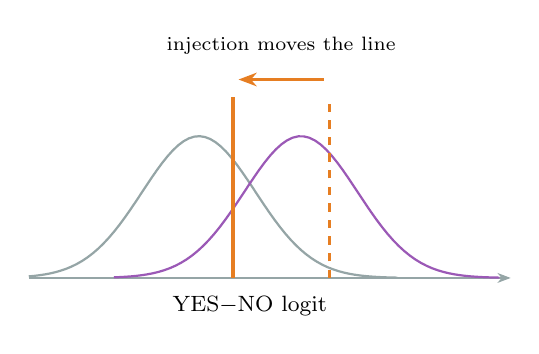
\begin{tikzpicture}[scale=0.72]
  \draw[-{Stealth},neutral] (-3,0) -- (5.5,0);
  \draw[thick,neutral,domain=-3:3.5,samples=70] plot (\x,{2.5*exp(-(\x)^2/2)});
  \draw[thick,state,domain=-1.5:5.3,samples=70] plot (\x,{2.5*exp(-(\x-1.8)^2/2)});
  \draw[bias,very thick,dashed] (2.3,0) -- (2.3,3.2);
  \draw[bias,very thick] (0.6,0) -- (0.6,3.2);
  \draw[-{Stealth},bias,thick] (2.2,3.5) -- (0.7,3.5);
  \node[font=\scriptsize,text=black,align=center] at (1.45,4.1) {injection moves the line};
  \node[font=\footnotesize,text=black] at (0.9,-0.5) {YES$-$NO logit};
\end{tikzpicture}
\end{column}
\begin{column}{0.48\textwidth}
{\small \href{\site/papers/hahami-2025/}{Hahami et al.\ (2025)} read the YES-minus-NO logit in Llama-3.1-8B-Instruct. They apply the same injection to control questions whose answer is no.

\vspace{0.4em}
The rise on the detection question and the rise on the controls correlate at $\mathbf{r = 0.999}$.}
\end{column}
\end{columns}

\vspace{0.5em}
In signal detection terms, the injection shifts the \textbf{\textcolor{bias}{criterion}}: the model becomes more likely to say yes to any question.

\vspace{0.3em}
{\small Lindsey's check on unrelated questions in Claude models finds no increase in yes answers.}
\end{frame}

\begin{frame}[label=logit]{A logit as a decision variable}
\begin{columns}[T]
\begin{column}{0.5\textwidth}
\begin{center}
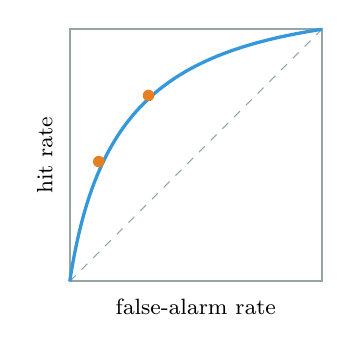
\begin{tikzpicture}[scale=0.8]
  \draw[neutral,thick] (0,0) rectangle (4,4);
  \draw[neutral,dashed] (0,0) -- (4,4);
  \draw[report,very thick] (0,0) .. controls (0.4,2.6) and (1.4,3.6) .. (4,4);
  \foreach \p in {(0.46,1.9),(1.25,2.95)} \fill[bias] \p circle (2.6pt);
  \node[font=\footnotesize,text=black] at (2,-0.4) {false-alarm rate};
  \node[font=\footnotesize,text=black,rotate=90] at (-0.4,2) {hit rate};
\end{tikzpicture}
\end{center}
\end{column}
\begin{column}{0.48\textwidth}
{\small
\textcolor{bias}{\textbf{Rating scale:}} a few criteria, so a few points on the ROC curve (orange dots).

\vspace{0.5em}
\textcolor{report}{\textbf{Logit difference:}} continuous. Every possible threshold is a criterion, so the full receiver operating characteristic curve (blue) comes from one run, without asking for ratings.

\vspace{0.5em}
Hahami et al.\ read every answer this way.
}
\end{column}
\end{columns}
\end{frame}

\begin{frame}[label=conftasks]{Confidence papers as type-2 tasks}
Three papers score a model's confidence against its own correctness:

\vspace{0.5em}
\begin{center}
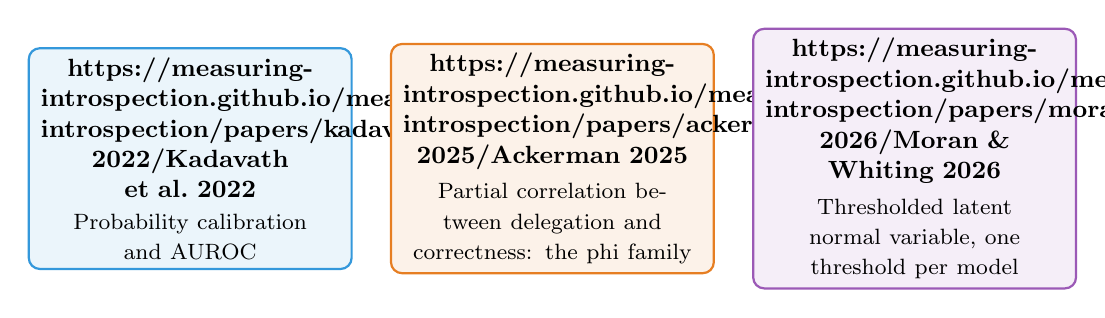
\begin{tikzpicture}
  \node[box=report,minimum width=4.1cm,minimum height=2.3cm,text width=3.8cm] at (0,0) {\textbf{\href{\site/papers/kadavath-2022/}{Kadavath et al.\ 2022}}\\[0.2em]{\footnotesize Probability calibration\\and AUROC}};
  \node[box=bias,minimum width=4.1cm,minimum height=2.3cm,text width=3.8cm] at (4.6,0) {\textbf{\href{\site/papers/ackerman-2025/}{Ackerman 2025}}\\[0.2em]{\footnotesize Partial correlation between delegation and correctness: the phi family}};
  \node[box=state,minimum width=4.1cm,minimum height=2.3cm,text width=3.8cm] at (9.2,0) {\textbf{\href{\site/papers/moran-2026/}{Moran \& Whiting 2026}}\\[0.2em]{\footnotesize Thresholded latent normal variable, one threshold per model}};
\end{tikzpicture}
\end{center}

\vspace{0.5em}
{\small Ackerman's measure is in the \hyperlink{fail}{phi family}, which moves with bias. Moran and Whiting's threshold separates a model's yes rate from the shared signal; they state that the normality assumption is presumed rather than tested.}
\end{frame}

\begin{frame}[label=probe]{A probe as the ideal observer}
\relax{\small Meta-$d'$ compares confidence with the evidence the decision had. The closest LLM version compares the model's report with a probe trained on the same activations.}

\vspace{0.2em}
\begin{center}
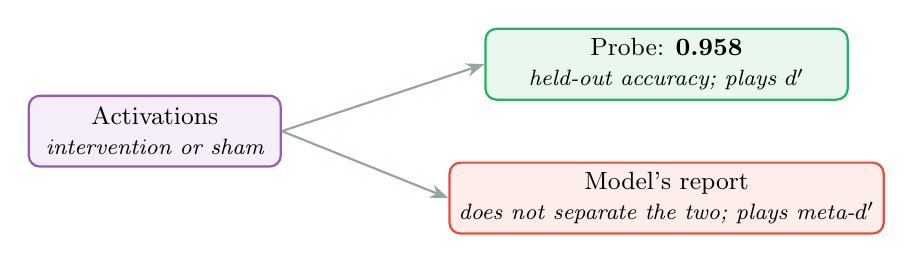
\begin{tikzpicture}
  \node[box=state] (act) at (0,0) {Activations\\{\footnotesize\itshape intervention or sham}};
  \node[box=pass,minimum width=4.6cm] (probe) at (6.5,0.85) {Probe: \textbf{0.958}\\{\footnotesize\itshape held-out accuracy; plays $d'$}};
  \node[box=fail,minimum width=4.6cm] (rep) at (6.5,-0.85) {Model's report\\{\footnotesize\itshape does not separate the two; plays meta-$d'$}};
  \draw[-{Stealth},thick,neutral] (act.east) -- (probe.west);
  \draw[-{Stealth},thick,neutral] (act.east) -- (rep.west);
\end{tikzpicture}
\end{center}

\vspace{0.2em}
{\small \href{\site/papers/ferrara-2026/}{Ferrara (2026)}, Qwen2.5-7B-Instruct. Ferrara defines the ratio of report margin to probe margin as an M-ratio analog.}

\vspace{0.2em}
{\small In plain terms: the information is in the activations, and it does not reach the report.}
\end{frame}

%% ============================================================
\partslide{part5}{Part 5\\[0.5em]{\large\mdseries Limits}}
%% ============================================================

\begin{frame}[label=limits]{Where the analogy stops}
\begin{itemize}\setlength\itemsep{8pt}
  \item {\small \textbf{Items, not internal noise.} Signal detection's standard design holds the stimulus constant, so variation in answers reflects noise inside the observer (\FL). Many LLM experiments sample at temperature 0, where an item always gets the same answer. Variation then comes from items, and $d'$ describes distributions over items.}
  \item {\small \textbf{One subject.} Human studies estimate efficiency per subject and compare subjects. A model sampled many times is one subject, and differences between models mix architecture, training and prompt format.}
  \item {\small \textbf{Type-1 and type-2 can merge.} Meta-$d'$ rests on a model of the type-1 decision. In an LLM the confidence prompt can make the model solve the item again. Moran and Whiting report that reasoning-trained models often do, which turns a type-2 judgment into a second type-1 attempt.}
\end{itemize}
\end{frame}

\begin{frame}[label=summary]{Summary}
\begin{center}
{\footnotesize\renewcommand{\arraystretch}{1.02}
\begin{tabular}{L{3.6cm}L{6.2cm}L{2.8cm}}
\toprule
\textbf{Idea} & \textbf{Question for an introspection experiment} & \textbf{Card stage} \\
\midrule
Hits and false alarms & Is the yes rate without injection reported? & Instrument \\
$d'$ versus criterion & Is a yes-bias separated from sensitivity? & Measurement model \\
Empty cells & Which correction is used when $F = 0$? & Uncertainty \\
Type-1 versus type-2 & Is the task about the world or the model's answer? & Measurement model \\
Sensitivity, bias, efficiency & Which of the three does the measure track? & Measurement model \\
AUROC2 and Brier score & Does the number move with task performance? & Uncertainty \\
Three calibrations & Which sense of calibration is meant? & Calibration \\
Meta-$d'$ and the probe & Is the report compared with a probe? & Comparability \\
Constant stimuli & Does variation come from items or the model? & Validity conditions \\
\bottomrule
\end{tabular}
}
\end{center}
\end{frame}

\begin{frame}[label=reading]{Reading}
\small
\begin{itemize}
  \item \href{https://www.frontiersin.org/articles/10.3389/fnhum.2014.00443/pdf}{Fleming \& Lau, How to measure metacognition} (2014): sensitivity, bias and efficiency; bias-free measures; the Brier decomposition.
  \item \href{https://www.sciencedirect.com/science/article/abs/pii/S1053810011002303}{Maniscalco \& Lau, A signal detection theoretic approach for estimating metacognitive sensitivity from confidence ratings} (2012): meta-$d'$.
  \item \href{https://www.columbia.edu/~bsm2105/type2sdt/}{Maniscalco, type-2 SDT code}: fitting meta-$d'$.
  \item \href{https://philarchive.org/archive/MICCIC-3}{Michel, Confidence in consciousness research} (2023): validity versus accuracy; conditions and confounds.
  \item \href{https://philpapers.org/archive/MICTOA-2.pdf}{Michel, The old and new criterion problems} (2023): response bias in type-1 reports.
  \item \href{\site/foundations/signal-detection/}{Signal detection and metacognition}: the site page this deck follows.
\end{itemize}
\end{frame}

\end{document}
